% Created 2018-01-14 Sun 16:41
% Intended LaTeX compiler: pdflatex
\documentclass[11pt]{article}
\usepackage[utf8]{inputenc}
\usepackage[T1]{fontenc}
\usepackage{graphicx}
\usepackage{grffile}
\usepackage{longtable}
\usepackage{wrapfig}
\usepackage{rotating}
\usepackage[normalem]{ulem}
\usepackage{amsmath}
\usepackage{textcomp}
\usepackage{amssymb}
\usepackage{capt-of}
\usepackage{hyperref}
\usepackage{minted}
\usepackage{fancyhdr}
\setcounter{secnumdepth}{-1} 
\pagestyle{fancy}
\fancyhead{} 
\rhead{\textit{Michael Laufer}}
\lhead{\textit{Numerical Methods Fall 2017, HW6}}
\small

\author{Michael Laufer}
\date{\today}
\title{Project Proposal Methods Fall 2017}
\hypersetup{
 pdfauthor={Michael Laufer},
 pdftitle={Project Proposal Methods Fall 2017},
 pdfkeywords={},
 pdfsubject={},
 pdfcreator={Emacs 25.3.1 (Org mode 9.1.4)}, 
 pdflang={English}}
\begin{document}

\maketitle
\section{Steady State Thermal Simulation of a 2D Heatpipe-based Cooler for Mobile Processors}
\label{sec:orgd18ea0b}
This project will attempt to predict the temperature distribution of a characteristic heatpipe based cooler for mobile processors. A cooler of this type is generally comprised of a copper contactor plate and a fin array connected with a super-high effective thermal conductivity element known as a heatpipe. The main challenge in this project will be to modify the Unspy code and implement the new boundary conditions characteristic of the problem. An accurate simulation of this type of cooler has many potential uses in industry that I will elaborate more on in my final project.
A basic heatpipe-based cooler can be seen in the following image:
\begin{center}
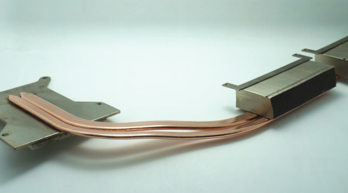
\includegraphics[width=.9\linewidth]{./figures/heatpipe.png}
\end{center}   \newpage
In this work I plan to modify and fine-tune the generic Finite Volume Method solver code that was provided to us in the class.  After analyzing the code given along with the physics of the problem at hand, a number of modifications and new elements must be added to the solver. 
Some of these additions include:
\begin{itemize}
\item Explicitly setting the diffusion coefficient (the code implies a value of 1)
\item Implementing non-uniform diffusion coefficient
\item Implementing the inverse distance-weighted harmonic mean formula for calculating the diffusion coefficient at the faces (needed for dealing with the discontinuous thermal conductivity in the problem).
\item Adding convective heat transfer BC
\item Adding adiabatic BC
\item Verifying Neuman BC for use as a specified heat flux.
\item Accelerate the code with a python JIT compiler such as Numba, to allow for much speedier execution. This is a needed step for future use as a base for an unsteady solver.
\end{itemize}
An additional challenge will be to build the complex geometry and mesh within gmsh.
To validate and check the work done in this project, an identical heat transfer simulation will be setup using an industry standard Finite Element solver with the same BCs. The two solutions will be compared as well as the solving time needed for convergence.
\end{document}